\documentclass{seminar}
\usepackage{epic,/homes/tiwari/Talks/Special/relative,latexsym,url}
\usepackage{/homes/tiwari/Talks/Special/gastex}
\usepackage{wrapfig}

\usepackage{fancybox}
\usepackage{semlayer}
\usepackage{epsfig}
\usepackage{amssymb}
\usepackage{semcolor}

\def\printlandscape{\special{landscape}}    % Works with dvips.
\renewcommand{\printlandscape}{\special{landscape}}
\special{! /landplus90 true store}

\input{/homes/tiwari/Talks/Special/slideprel}
\slideframe{oval}
\usepackage{times} 		%% for PDF purposes

\newcommand\ignore[1]{{{}}}

% \ifpdf\else
%%%%%%%%
% to fix problems making landscape seminar pdfs
% Letter...
%\pdfpagewidth=11truein
%\pdfpageheight=8.5truein
% A4
\pdfpagewidth=297truemm % your milage may vary....
\pdfpageheight=210truemm
\pdfhorigin=1truein     % default value(?), but doesn't work without
\pdfvorigin=1truein     % default value(?), but doesn't work without
%\fi
% -------------------------------------------------------

%---------------------------------------------------------------------
\begin{document}
%---------------------------------------------------------------------
\begin{slide}
\heading{Relational Abstraction: A new abstraction concept}

\begin{tabular}{c|c}
\begin{minipage}{1.8in}
\begin{description}
\item[Benefit:] Enables analyzability of complex systems
\\
\hspace*{-3em}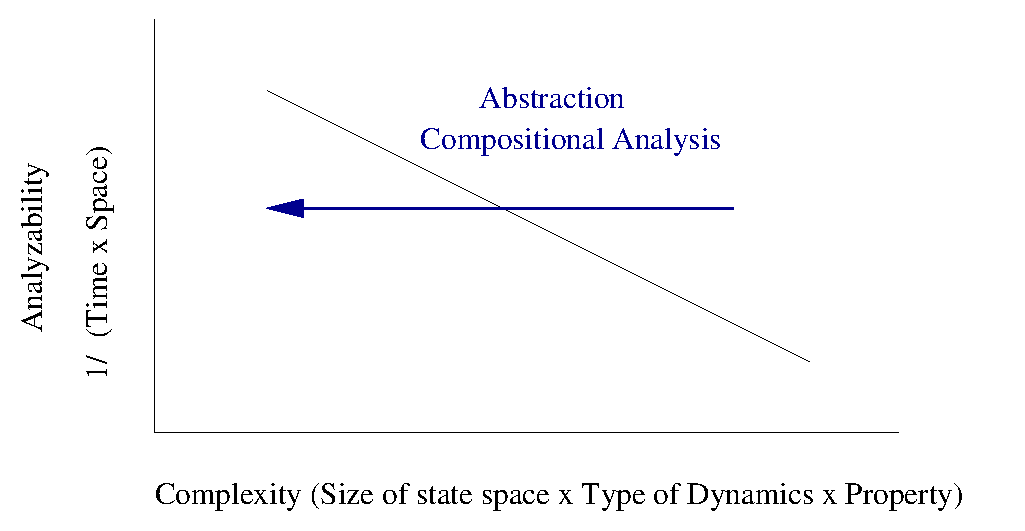
\includegraphics[angle=0,scale=0.3]{reduceComplexity}

\item[Feature:] Compositional analysis: Abstracts open components
 with hybrid dynamics

\item[Feature:] Compatible with other abstraction and model checking
 techniques
\end{description}
\end{minipage}
&
\begin{minipage}{2.1in}
\begin{description}
\item[Novelty:] Abstracts the transition relation, not the state space
\\
\hspace*{-2em}
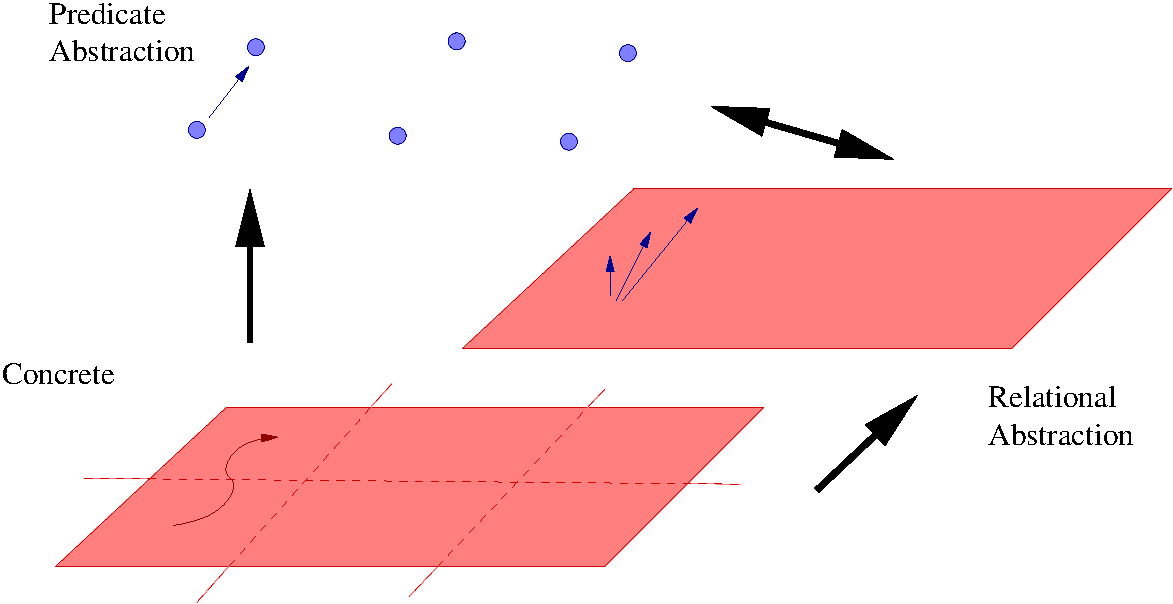
\includegraphics[angle=0,scale=0.35]{relabs}

\item[Scope:] Applies to all dynamical systems. Effective relational
 abstractions can be computed for several classes.
\end{description}
\end{minipage}
\end{tabular}

\end{slide}
% -------------------------------------------------------
\begin{slide}
\subheading{Relational Abstraction: Examples}

\begin{tabular}{c|c|c}
\begin{minipage}{1.3in}
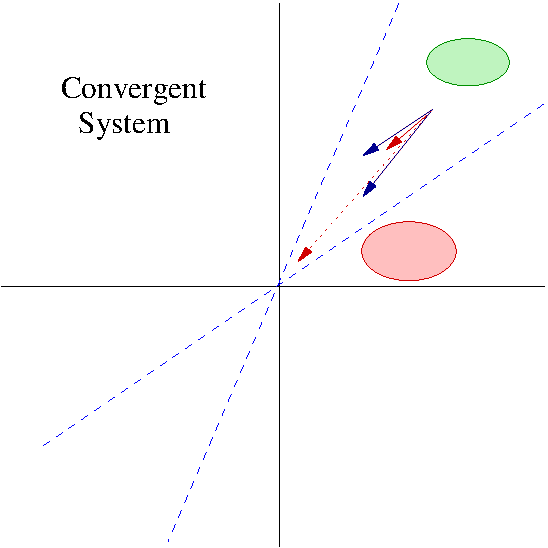
\includegraphics[angle=0,scale=0.3]{conv}
\\
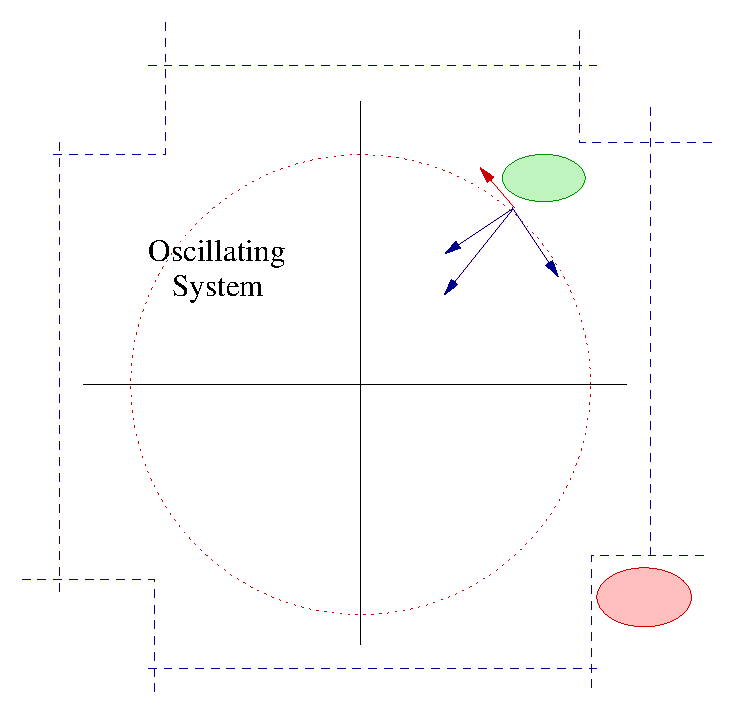
\includegraphics[angle=0,scale=0.3]{osci}
\end{minipage}
&
\begin{minipage}{1.2in}
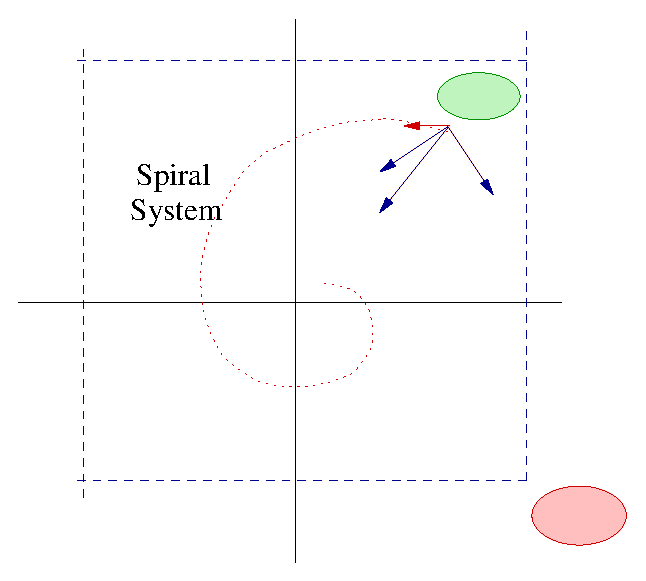
\includegraphics[angle=0,scale=0.3]{spiral}
\\
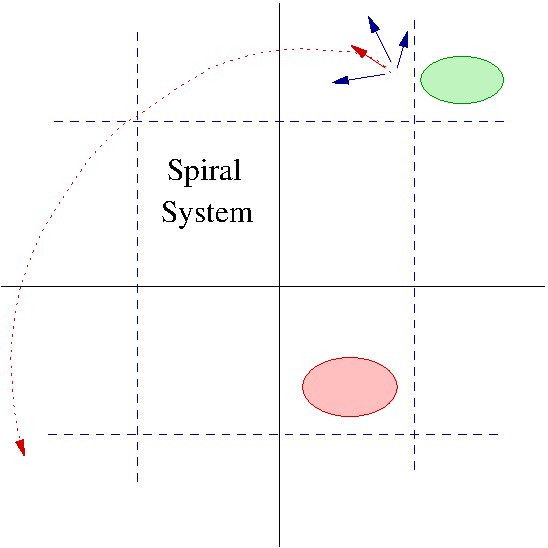
\includegraphics[angle=0,scale=0.3]{spiral-out}
\end{minipage}
&
\begin{minipage}{1.4in}
\small{
\begin{tabular}{|p{0.34in}|p{0.33in}|p{0.33in}|}
\hline
Class & $\frac{d\vec{x}}{dt}$ & RelAbs
\\
\hline \hline
\parbox{0.34in}{Timed System} & 
\parbox{0.34in}{$\dot{x}=1$,\\$\dot{y} = 1$} & 
\parbox{0.45in}{$x'-x=\\y'-y$}
\\
\hline
\parbox{0.34in}{Multirate System} & 
\parbox{0.34in}{$\dot{x}=2$,\\$\dot{y}=3$} & 
\parbox{0.33in}{$\frac{x'-x}{2} = \\ \frac{y'-y}{3}$}
\\
\hline
\parbox{0.34in}{Linear Hybrid System} & 
\parbox{0.36in}{$\dot{\vec{x}} = A\vec{x}$} & 
\parbox{0.33in}{$(0 \leq p'\leq p$}
\\
\hline
$\ldots$ & $\ldots$ & $\ldots$
\\
\hline
\end{tabular}

\bigskip

On Hybrid System benchmarks, verification time reduces from
~{\cem{10 hours}} to a {\cem{few minutes}} ({\crm{100x}} improvement).
}
\end{minipage}
\end{tabular}

\end{slide}
% -------------------------------------------------------
\end{document}
